\chapter{Praktische uitwerking Kotlin Native}
\label{ch:praktisch}
In dit hoofdstuk zal er praktisch een Kotlin Native project worden gebouwd. De bedoeling is om aan de hand van een voorbeeld de volledige werking uit te leggen. In dit voorbeeld zal er een simpele applicatie gebouwd worden waarbij gebruikers een shopping cart kunnen aanmaken, producten kunnen bekijken en toevoegen aan de shopping cart en kunnen afrekenen.

\section{Domeinmodel}
Aangezien het doel van Kotlin Native het delen van business logica is, is het handig om op voorhand na te denken over het domeinmodel. Welke klassen heb ik nodig, welke attributen en methodes moeten deze klassen hebben. Een domeinmodel geeft je ook een duidelijk overzicht over je applicatie.

TOEVOEGEN FOTO

\section{Requirements}
Om gebruik te kunnen maken van Kotlin Native voor het ontwikkelen van cross-platform applicaties (iOS \& Android), zijn er enkele vereisten:
\begin{itemize}
	\item \textbf{Android studio} voor het ontwikkelen van de Android applicatie.
	\item \textbf{Xcode} voor het ontwikkelen van de iOS applicatie (toestel met MacOS is vereist).
	\item \textbf{IntelliJ IDEA} (optioneel) voor het opzetten van het project. Dit kan eventueel met een andere IDEA die gradle projecten ondersteunt, worden opgezet.
	\item \textbf{Gradle} om gebruik te kunnen maken van de Kotlin Native compiler en plugin. Deze wordt geïnstalleerd bij het instellen van IntelliJ IDEA of Android Studio.
\end{itemize}

\section{Stap 1: project initiatie}
De eerste stap in het ontwikkelen van een Kotlin Native project is het maken van een nieuwe map, op een gewenste locatie op de harde schijf van je computer. Hierin zal er een eerste bestand worden aangemaakt: \textbf{build.gradle}.

\begin{lstlisting}
subprojects {
 buildscript {
  ext.kotlin_version = '1.2.31'
  ext.kotlin_native_version = '0.6.2'
		
  repositories {
   jcenter()
   google()
   maven { url "http://kotlin.bintray.com/kotlinx" }
   maven { url "https://plugins.gradle.org/m2/" }
   maven { url "https://dl.bintray.com/jetbrains/ kotlin-native-dependencies" }
  }

  dependencies {
   classpath "org.jetbrains.kotlin:kotlin-gradle-plugin: $kotlin_version"
   classpath 'com.android.tools.build:gradle:3.0.1'
   classpath "org.jetbrains.kotlin:kotlin-native-gradle-plugin: $kotlin_native_version"
  }
 }
	
 group 'ilias.vw'
 version '1.0-SNAPSHOT'
	
 repositories {
  jcenter()
  maven { url "http://kotlin.bintray.com/kotlinx" }
 }
	
 tasks.withType(Test) {
  testLogging {
   showStandardStreams = true
   events "passed", "failed"
  }
 }
}
\end{lstlisting}
\subsection{Versies}
Bovenaan geven we aan welke versie van Kotlin en Kotlin Native we willen gebruiken. Dit zijn beide de nieuwste versies. Opgelet, het is niet altijd vanzelfspreken om de laatste versie van Kotlin Native te gebruiken. Er wordt voortdurend gewerkt aan Kotlin Native en nieuwe dingen worden continu gepushed op de Github repository. Het kan al eens gebeuren dat sommige dingen niet altijd even goed werken, waardoor de applicatie soms niet werkt. Bij twijfels, neem een minder recente versie van de Kotlin Native plugin.

\subsection{Repositories}
In de repositories tag worden de juiste repositories gelinkt:
\begin{itemize}
	\item \textbf{Kotlinx} bevat alle coroutines\footnote{Programmaonderdelen die asynchroon programmeren vergemakkelijken door gecompliceerde logica in bibliotheken te steken} die Kotlin kan gebruiken.
	\item \textbf{Gradle}
	\item \textbf{Kotlin-native-dependencies} stelt alle dependencies die Kotlin Native nodig heeft ter beschikking.
\end{itemize}

\subsection{Dependencies}
In de dependencies tag worden de juiste dependencies gelinkt:
\begin{itemize}
	\item \textbf{Kotlin-gradle} laadt de juiste versie van Kotlin.
	\item \textbf{Android build tools} is nodig voor het bouwen van de Android applicatie.
	\item \textbf{Kotlin-native-gradle-plugin} is de Kotlin Native plugin die gebruikt zal worden om te zorgen voor een cross-platforme applicatie.
\end{itemize}

\subsection{Overige informatie}
\label{sec:overige}
\begin{itemize}
	\item \textbf{Group} stelt het groupId van het project in.
	\item \textbf{Version} geeft de versie van het project weer.
	\item \textbf{testLogging} wordt gebruikt voor het uitvoeren van de testen.
\end{itemize}

\section{Stap 2: project structuur}
Nadat het build.gradle bestand gemaakt is, is het de bedoeling om via IntelliJ IDEA het gradle bestand te importeren. Zie figuur \ref{fig:stap2-import}. IntelliJ zal een dialoogvenster openen, waarbij het build.gradle bestand moet worden geopend. De IDE zal hierna het build.gradle bestand uitvoeren en het genereert enkele bestanden.

\begin{figure} [ht]
	\centering
	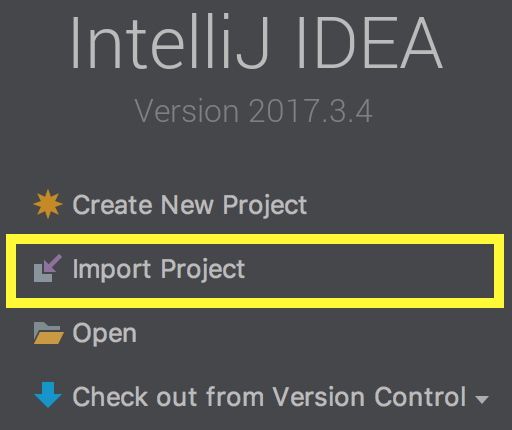
\includegraphics[width=0.60\textwidth]{img/stap2-import.png}
	\caption{Importeren van een project}
	\label{fig:stap2-import}
\end{figure}

In de huidige versie van Kotlin Native worden de overige folders (nog?) niet automatisch aangemaakt. Alle andere folders, die te zien zijn in figuur \ref{fig:knstructuur} moeten handmatig gemaakt worden.

\section{Stap 3: Common folder }
In de common folder wordt alle gemeenschappelijke code aangemaakt. In deze folder moet er aan een bepaalde structuur worden voldaan, zie figuur \ref{fig:stap3-common}.

\begin{figure} [ht]
	\centering
	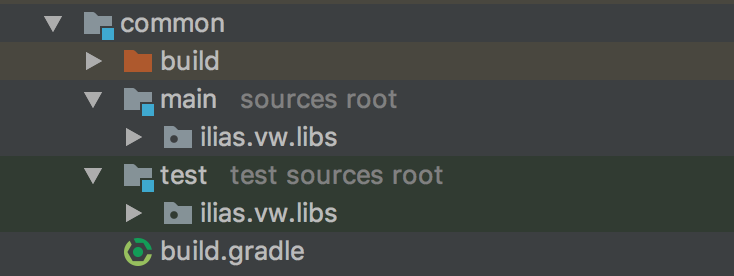
\includegraphics[width=0.60\textwidth]{img/stap3-common.png}
	\caption{Common module structuur}
	\label{fig:stap3-common}
\end{figure}

\subsection{Build folder}
De build folder bevat alle gecompileerde bestanden die genereerd worden door Kotlin Native. Deze bestanden worden aangemaakt bij iedere gradle run en/of build.

\subsection{Main en test folder}
Zoals te zien is op figuur \ref{fig:stap3-common} heeft zowel de main als test folder enkele subpackages. Deze beginnen met de groupId die ingesteld is in sectie \ref{sec:overige} met daarin nog eens een 'libs' folder. De naam van deze 'libs' folder is vrij te kiezen.

De main folder zal alle gemeenschappelijke klassen bevatten (expect en gewone klassen, zie sectie \ref{sec:expectandactual}).

De test folder zal alle gemeenschappelijke test klassen bevatten, gebruikmakend van de klassen in de main folder.

\subsection{Build.gradle}
Natuurlijk moet de common module ook gecompileerd worden door Kotlin Native. Hiervoor is er een build.gradle nodig.

\begin{lstlisting}
apply plugin: 'kotlin-platform-common'

sourceSets {
 main.kotlin.srcDirs += 'main/'
 test.kotlin.srcDirs += 'test/'
}

dependencies {
 compile "org.jetbrains.kotlin:kotlin-stdlib-common:$kotlin_version"
 testCompile "org.jetbrains.kotlin:kotlin-test-annotations-common: $kotlin_version"
 testCompile "org.jetbrains.kotlin:kotlin-test-common:$kotlin_version"
}
\end{lstlisting}
De bovenste regel in de build.gradle geeft aan dat we gebruik maken van de kotlin-platform-common plugin. Deze zal verantwoordelijk zijn voor het compileren en delen van alle gemeenschappelijke code over de verschillende platformen.

Er worden ook twee sourceSets toegevoegd. SourceSets vertegenwoordigen een logische groep van Java en/of Kotlin bronnen en middelen.

Tenslotte worden er drie dependencies toegevoegd. De stdlib is verantwoordelijk voor het aanmaken van de Kotlin Standard Library. Er worden nog twee test dependencies toegevoegd, één verantwoordelijk voor de annotations, de andere voor het opstellen en uitvoeren van de testen (later meer over testen).

CODE TOEVOEGEN!!

\section{Stap 4: platforms folder}

\section{Stap 5: Android folder}

\section{Stap 6: iOS folder}
%Vergeet niet de build phases en scripts%

\section{Optioneel: testen}

\section{User interfaces}